\RequirePackage{etex}
\documentclass[margin=0.1cm,varwidth=\maxdimen]{standalone}
\usepackage{fontawesome5}
\usepackage[usenames]{color}
\usepackage{amssymb}
\usepackage{amsmath}
\usepackage[utf8]{inputenc}
\usepackage{tikz}
\usetikzlibrary{arrows, calc, decorations.pathmorphing, decorations.pathreplacing, calligraphy, backgrounds, math, shapes, shapes.geometric, spy, positioning}
\usepackage{tikz-network}
\usepackage{pgfplots}
\usepackage{pgfplotstable}
\pgfplotsset{compat=1.17}
\usepackage{graphicx}
\usepackage{multirow}
\usepackage{xxcolor}

\begin{document}

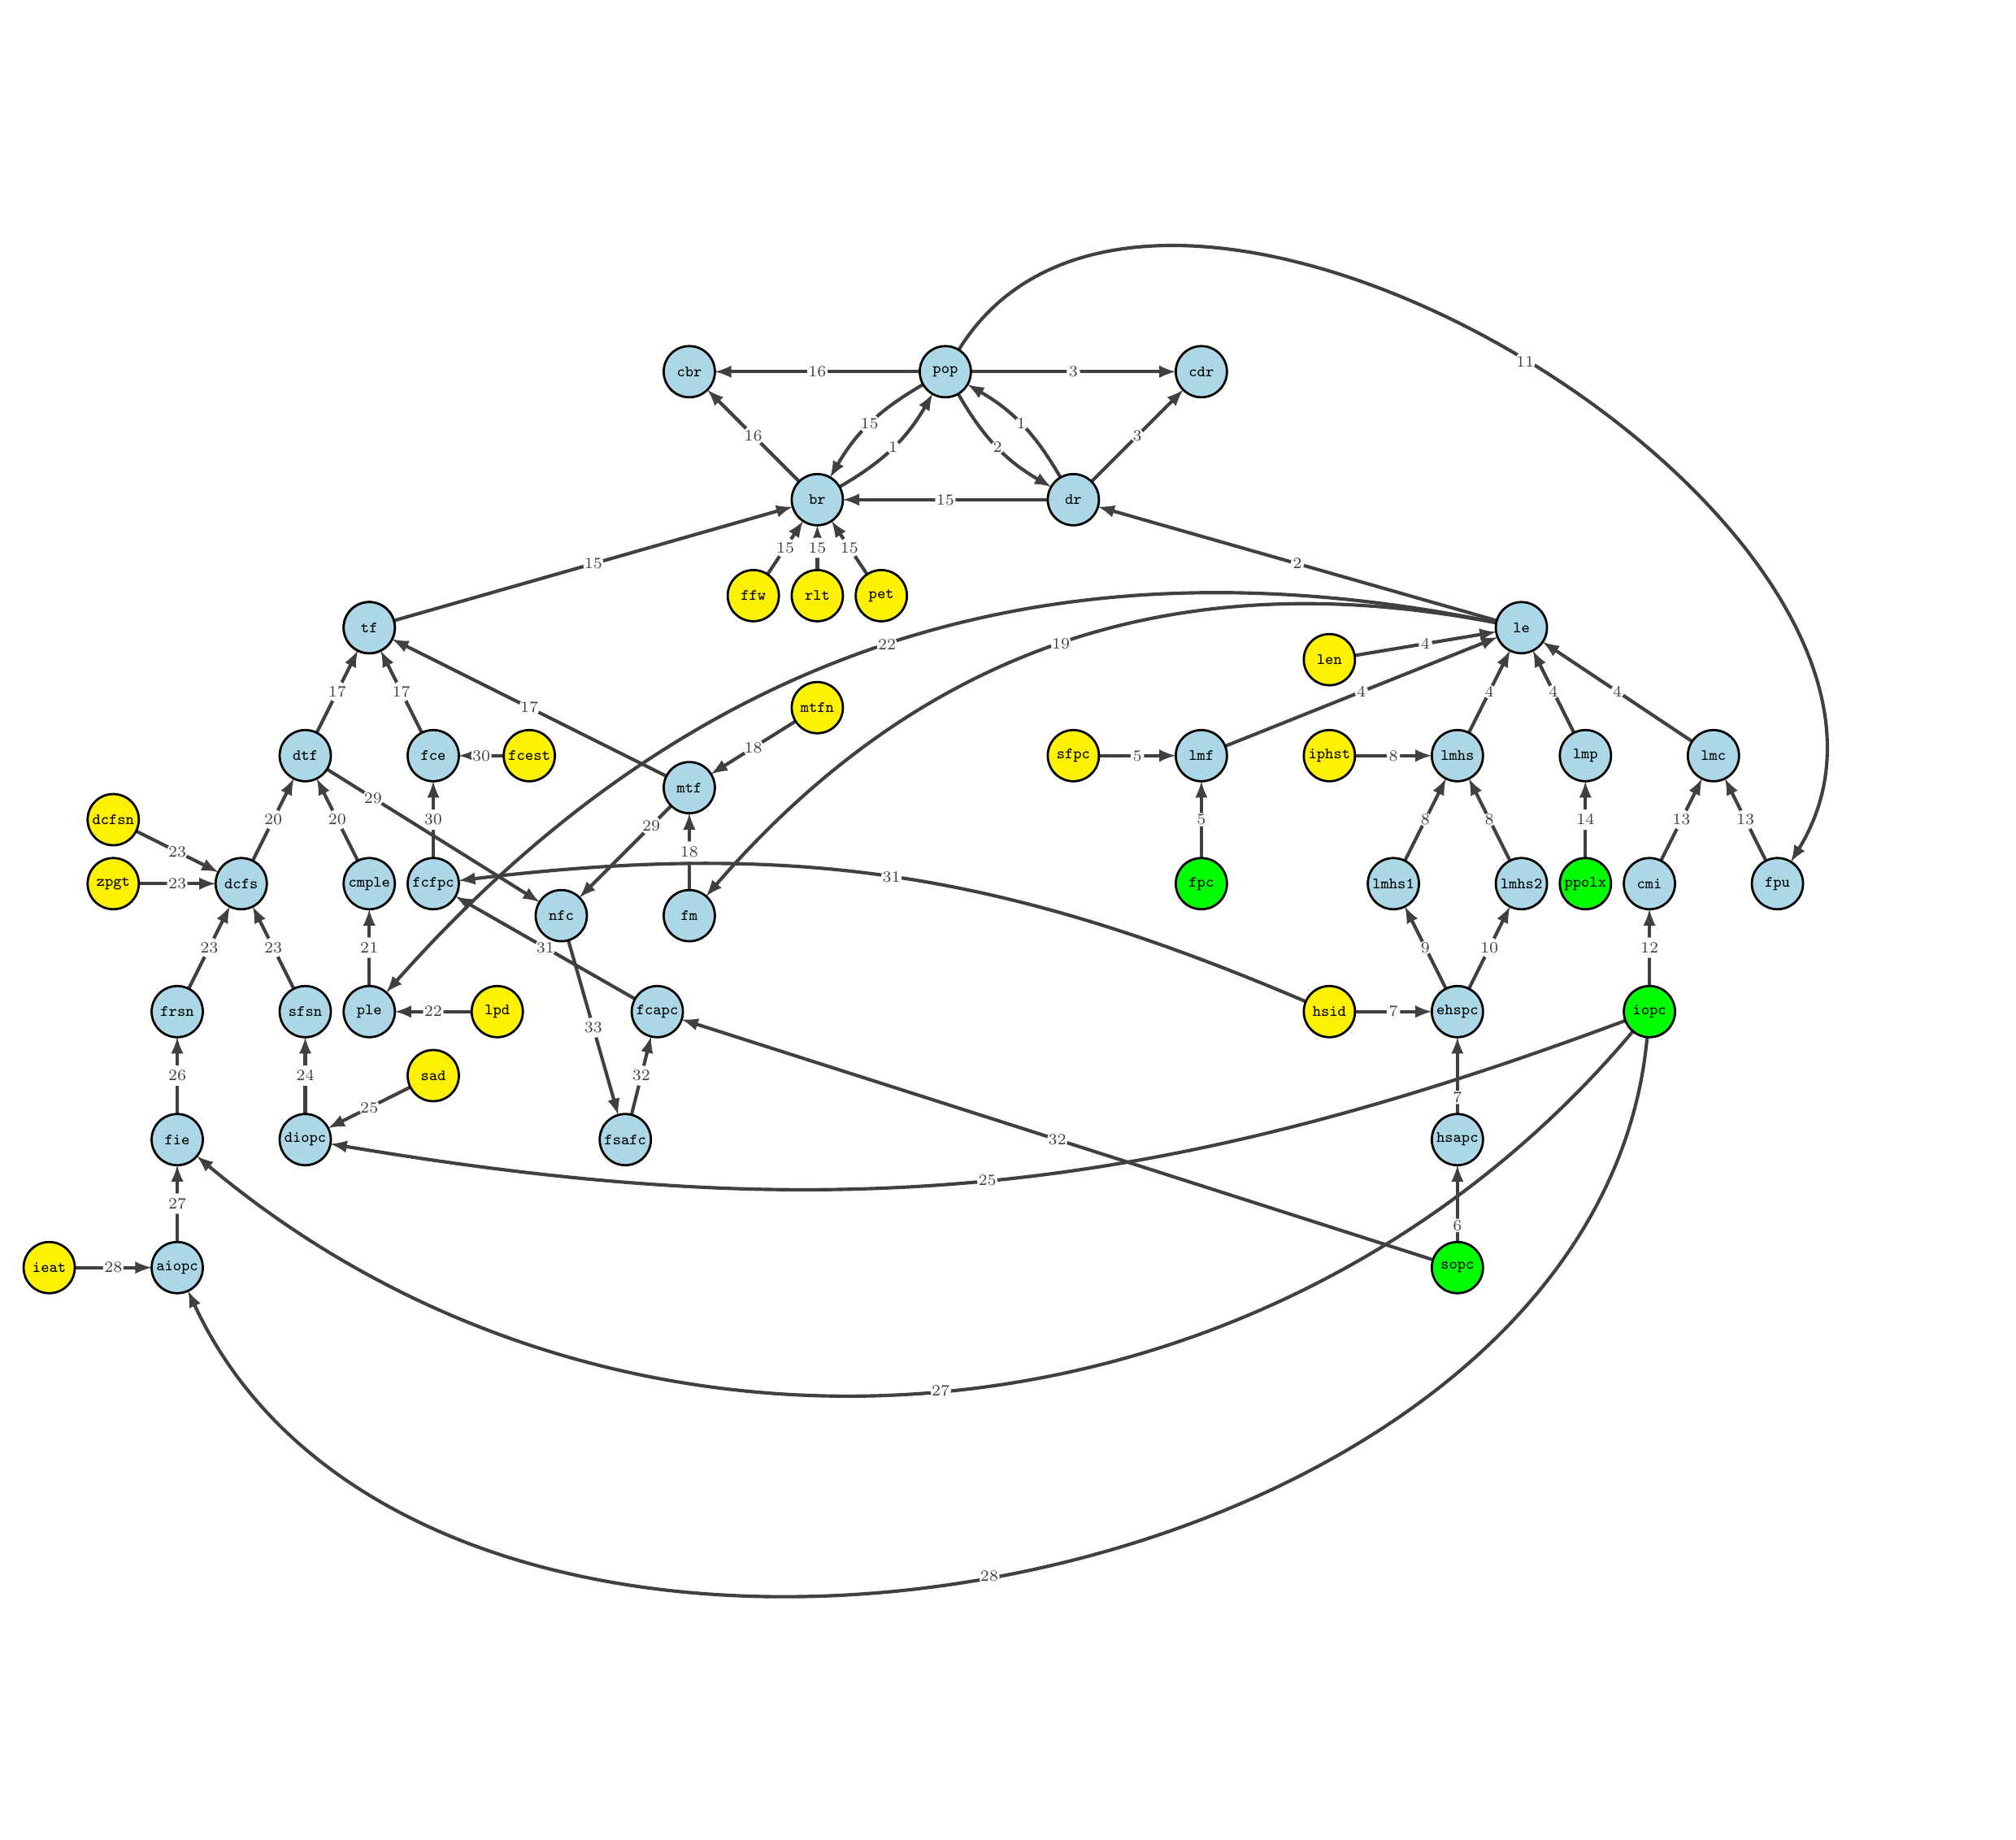
\begin{tikzpicture}
  \SetVertexStyle[MinSize=0.8\DefaultUnit]
  % Population variables and parameters
  \Vertex[x=0,y=0,label=\texttt{pop}]{pop}
  \Vertex[x=-2,y=-2,label=\texttt{br}]{br}
  \Vertex[x=2,y=-2,label=\texttt{dr}]{dr}
  % Death rate variables and parameters
  \Vertex[x=4,y=0,label=\texttt{cdr}]{cdr}
  \begin{scope}[xshift=7cm]
  \Vertex[x=2,y=-4,label=\texttt{le}]{le}
  \Vertex[x=-1,y=-4.5,label=\texttt{len},color=yellow]{len}
  \Vertex[x=-3,y=-6,label=\texttt{lmf}]{lmf}
  \Vertex[x=1,y=-6,label=\texttt{lmhs}]{lmhs}
  \Vertex[x=-1,y=-6,label=\texttt{iphst},color=yellow]{iphst}
  \Vertex[x=0,y=-8,label=\texttt{lmhs1}]{lmhs1}
  \Vertex[x=2,y=-8,label=\texttt{lmhs2}]{lmhs2}
  \Vertex[x=3,y=-6,label=\texttt{lmp}]{lmp}
  \Vertex[x=3,y=-8,label=\texttt{ppolx},color=green]{ppolx}
  \Vertex[x=5,y=-6,label=\texttt{lmc}]{lmc}
  \Vertex[x=4,y=-8,label=\texttt{cmi}]{cmi}
  \Vertex[x=4,y=-10,label=\texttt{iopc},color=green]{iopc}
  \Vertex[x=6,y=-8,label=\texttt{fpu}]{fpu}
  \Vertex[x=-3,y=-8,label=\texttt{fpc},color=green]{fpc}
  \Vertex[x=-5,y=-6,label=\texttt{sfpc},color=yellow]{sfpc}
  \Vertex[x=1,y=-10,label=\texttt{ehspc}]{ehspc}
  \Vertex[x=-1,y=-10,label=\texttt{hsid},color=yellow]{hsid}
  \Vertex[x=1,y=-12,label=\texttt{hsapc}]{hsapc}
  \Vertex[x=1,y=-14,label=\texttt{sopc},color=green]{sopc}
  \end{scope}
  % Birth rate variables and parameters
  \Vertex[x=-3,y=-3.5,label=\texttt{ffw},color=yellow]{ffw}
  \Vertex[x=-2,y=-3.5,label=\texttt{rlt},color=yellow]{rlt}
  \Vertex[x=-1,y=-3.5,label=\texttt{pet},color=yellow]{pet}
  \Vertex[x=-4,y=0,label=\texttt{cbr}]{cbr}
  \begin{scope}[xshift=-7cm]
  \Vertex[x=-2,y=-4,label=\texttt{tf}]{tf}
  \Vertex[x=-2,y=-4,label=\texttt{tf}]{tf}
  \Vertex[x=3,y=-6.5,label=\texttt{mtf}]{mtf}
  \Vertex[x=5,y=-5.25,label=\texttt{mtfn},color=yellow]{mtfn}
  \Vertex[x=3,y=-8.5,label=\texttt{fm}]{fm}
  \Vertex[x=1,y=-8.5,label=\texttt{nfc}]{nfc}
  \Vertex[x=-1,y=-6,label=\texttt{fce}]{fce}
  \Vertex[x=0.5,y=-6,label=\texttt{fcest},color=yellow]{fcest}
  \Vertex[x=-1,y=-8,label=\texttt{fcfpc}]{fcfpc}
  \Vertex[x=2.5,y=-10,label=\texttt{fcapc}]{fcapc}
  \Vertex[x=2,y=-12,label=\texttt{fsafc}]{fsafc}
  \Vertex[x=-3,y=-6,label=\texttt{dtf}]{dtf}
  \Vertex[x=-4,y=-8,label=\texttt{dcfs}]{dcfs}
  \Vertex[x=-6,y=-8,label=\texttt{zpgt},color=yellow]{zpgt}
  \Vertex[x=-6,y=-7,label=\texttt{dcfsn},color=yellow]{dcfsn}
  \Vertex[x=-5,y=-10,label=\texttt{frsn}]{frsn}
  \Vertex[x=-5,y=-12,label=\texttt{fie}]{fie}
  \Vertex[x=-5,y=-14,label=\texttt{aiopc}]{aiopc}
  \Vertex[x=-7,y=-14,label=\texttt{ieat},color=yellow]{ieat}
  \Vertex[x=-3,y=-10,label=\texttt{sfsn}]{sfsn}
  \Vertex[x=-3,y=-12,label=\texttt{diopc}]{diopc}
  \Vertex[x=-1,y=-11,label=\texttt{sad},color=yellow]{sad}
  \Vertex[x=-2,y=-8,label=\texttt{cmple}]{cmple}
  \Vertex[x=-2,y=-10,label=\texttt{ple}]{ple}
  \Vertex[x=0,y=-10,label=\texttt{lpd},color=yellow]{lpd}
  \end{scope}
  % Population dependencies
  \Edge[Direct,bend=-15,label=$1$](br)(pop)
  \Edge[Direct,bend=-15,label=$1$](dr)(pop)
  % Death rate dependencies
  \Edge[Direct,bend=-15,label=$2$](pop)(dr)
  \Edge[Direct,label=$2$](le)(dr)
  \Edge[Direct,label=$3$](pop)(cdr)
  \Edge[Direct,label=$3$](dr)(cdr)
  \Edge[Direct,label=$4$](len)(le)
  \Edge[Direct,label=$4$](lmf)(le)
  \Edge[Direct,label=$4$](lmhs)(le)
  \Edge[Direct,label=$4$](lmp)(le)
  \Edge[Direct,label=$4$](lmc)(le)
  \Edge[Direct,label=$5$](fpc)(lmf)
  \Edge[Direct,label=$5$](sfpc)(lmf)
  \Edge[Direct,label=$6$,distance=.2](sopc)(hsapc)
  \Edge[Direct,label=$7$,distance=.2](hsapc)(ehspc)
  \Edge[Direct,label=$7$](hsid)(ehspc)
  \Edge[Direct,label=$8$](lmhs1)(lmhs)
  \Edge[Direct,label=$8$](lmhs2)(lmhs)
  \Edge[Direct,label=$8$](iphst)(lmhs)
  \Edge[Direct,label=$9$](ehspc)(lmhs1)
  \Edge[Direct,label=$10$](ehspc)(lmhs2)
  \Edge[Direct,bend=90,label=$11$](pop)(fpu)
  \Edge[Direct,label=$12$](iopc)(cmi)
  \Edge[Direct,label=$13$](cmi)(lmc)
  \Edge[Direct,label=$13$](fpu)(lmc)
  \Edge[Direct,label=$14$](ppolx)(lmp)
  % Birth rate dependencies
  \Edge[Direct,label=$15$](dr)(br)
  \Edge[Direct,bend=-15,label=$15$](pop)(br)
  \Edge[Direct,label=$15$](ffw)(br)
  \Edge[Direct,label=$15$](rlt)(br)
  \Edge[Direct,label=$15$](pet)(br)
  \Edge[Direct,label=$15$](tf)(br)
  \Edge[Direct,label=$16$](pop)(cbr)
  \Edge[Direct,label=$16$](br)(cbr)
  \Edge[Direct,label=$17$](dtf)(tf)
  \Edge[Direct,label=$17$](fce)(tf)
  \Edge[Direct,label=$17$](mtf)(tf)
  \Edge[Direct,label=$18$](mtfn)(mtf)
  \Edge[Direct,label=$18$](fm)(mtf)
  \Edge[Direct,bend=-30,label=$19$](le)(fm)
  \Edge[Direct,label=$20$](dcfs)(dtf)
  \Edge[Direct,label=$20$](cmple)(dtf)
  \Edge[Direct,label=$21$](ple)(cmple)
  \Edge[Direct,bend=-30,label=$22$](le)(ple)
  \Edge[Direct,label=$22$](lpd)(ple)
  \Edge[Direct,label=$23$](dcfsn)(dcfs)
  \Edge[Direct,label=$23$](zpgt)(dcfs)
  \Edge[Direct,label=$23$](frsn)(dcfs)
  \Edge[Direct,label=$23$](sfsn)(dcfs)
  \Edge[Direct,label=$24$](diopc)(sfsn)
  \Edge[Direct,bend=15,label=$25$](iopc)(diopc)
  \Edge[Direct,label=$25$](sad)(diopc)
  \Edge[Direct,label=$26$](fie)(frsn)
  \Edge[Direct,bend=45,label=$27$](iopc)(fie)
  \Edge[Direct,label=$27$](aiopc)(fie)
  \Edge[Direct,bend=75,label=$28$](iopc)(aiopc)
  \Edge[Direct,label=$28$](ieat)(aiopc)
  \Edge[Direct,label=$29$,distance=.2](dtf)(nfc)
  \Edge[Direct,label=$29$,distance=.2](mtf)(nfc)
  \Edge[Direct,label=$30$](fcfpc)(fce)
  \Edge[Direct,label=$30$](fcest)(fce)
  \Edge[Direct,label=$31$](fcapc)(fcfpc)
  \Edge[Direct,bend=-15,label=$31$](hsid)(fcfpc)
  \Edge[Direct,label=$32$](sopc)(fcapc)
  \Edge[Direct,label=$32$](fsafc)(fcapc)
  \Edge[Direct,label=$33$](nfc)(fsafc)
\end{tikzpicture}

\end{document}
